\documentclass[conference]{IEEEtran}
\IEEEoverridecommandlockouts
\usepackage{cite}
\usepackage{amsmath,amssymb,amsfonts}
\usepackage{graphicx}
\usepackage{booktabs}
\usepackage{multirow}
\usepackage{xcolor}
\graphicspath{{figures/}}

\begin{document}

\title{A Comparative Study of RNN, LSTM, GRU and BiLSTM Models for Sentiment Analysis of IMDB Movie Reviews}

\author{\IEEEauthorblockN{Your Name}
\IEEEauthorblockA{\textit{Department of Computer Science and Engineering} \\
\textit{Your University Name}\\
City, India \\
your.email@university.edu}
}

\maketitle

\begin{abstract}
Sentiment analysis is a Natural Language Processing (NLP) task that automatically classifies the opinion expressed in a text as positive or negative. Since text is sequential data, recurrent neural networks (RNNs) are a natural choice for this task. This paper compares four recurrent architectures, namely SimpleRNN, Long Short-Term Memory (LSTM), Gated Recurrent Unit (GRU) and Bidirectional LSTM (BiLSTM), on the IMDB movie review dataset of 50,000 reviews, using identical preprocessing, embedding size, hidden units and training settings. The gated models clearly outperform the SimpleRNN (83.12\% accuracy). LSTM achieves the highest test accuracy of 86.76\%, BiLSTM achieves the highest F1-score of 0.867, and GRU reaches 85.54\% with fewer parameters. BiLSTM requires about $1.8\times$ the training time of LSTM without a significant accuracy gain. The study confirms that gating mechanisms reduce the vanishing gradient problem, and that LSTM or GRU give the best balance between accuracy and computational cost.
\end{abstract}

\begin{IEEEkeywords}
Sentiment analysis, recurrent neural network, LSTM, GRU, bidirectional LSTM, IMDB, deep learning, natural language processing
\end{IEEEkeywords}

\section{Introduction}
Online platforms generate huge volumes of user-written reviews and comments every day. Reading them manually is not feasible, so automatic sentiment analysis is widely used for product reviews, brand monitoring, customer support and recommendation systems. The main challenge is that the meaning of a sentence depends on word order and context. For example, ``not good'' has the opposite meaning of ``good''.

Feed-forward neural networks treat every input independently and cannot model this ordering. Recurrent Neural Networks (RNNs) address this by keeping a hidden state that carries information from previous time steps. However, a basic RNN suffers from the vanishing gradient problem~\cite{bengio1994} and forgets long-range context. LSTM~\cite{hochreiter1997} and GRU~\cite{cho2014} introduce gating mechanisms to address this, while bidirectional RNNs~\cite{schuster1997} process the sequence in both directions.

The contributions of this paper are:
\begin{itemize}
\item A controlled comparison of SimpleRNN, LSTM, GRU and BiLSTM for binary sentiment classification on IMDB, where only the recurrent layer differs between models.
\item An analysis of the trade-off between accuracy, model size and training time.
\item A qualitative analysis of model behaviour on mixed and negated sentences.
\end{itemize}

\section{Related Work}
Maas \textit{et al.}~\cite{maas2011} introduced the IMDB Large Movie Review dataset and learned word vectors for sentiment analysis. Hochreiter and Schmidhuber~\cite{hochreiter1997} proposed LSTM to learn long-term dependencies. Cho \textit{et al.}~\cite{cho2014} introduced the GRU within the RNN encoder--decoder framework, and Chung \textit{et al.}~\cite{chung2014} showed empirically that GRU and LSTM perform comparably on sequence modelling tasks. Schuster and Paliwal~\cite{schuster1997} proposed bidirectional RNNs. More recently, Transformer-based models such as BERT~\cite{devlin2019} achieve higher accuracy but require far more computation. This work focuses on lightweight recurrent models that can be trained on a standard CPU.

\section{Methodology}

\subsection{Dataset}
The IMDB dataset~\cite{maas2011} contains 50,000 movie reviews labelled positive or negative, with an equal number of each class. The standard split was used: 25,000 reviews for training, of which 20\% were held out for validation, and 25,000 reviews for testing. Fig.~\ref{fig:len} shows that most reviews are shorter than 300 words.

\begin{figure}[htbp]
\centerline{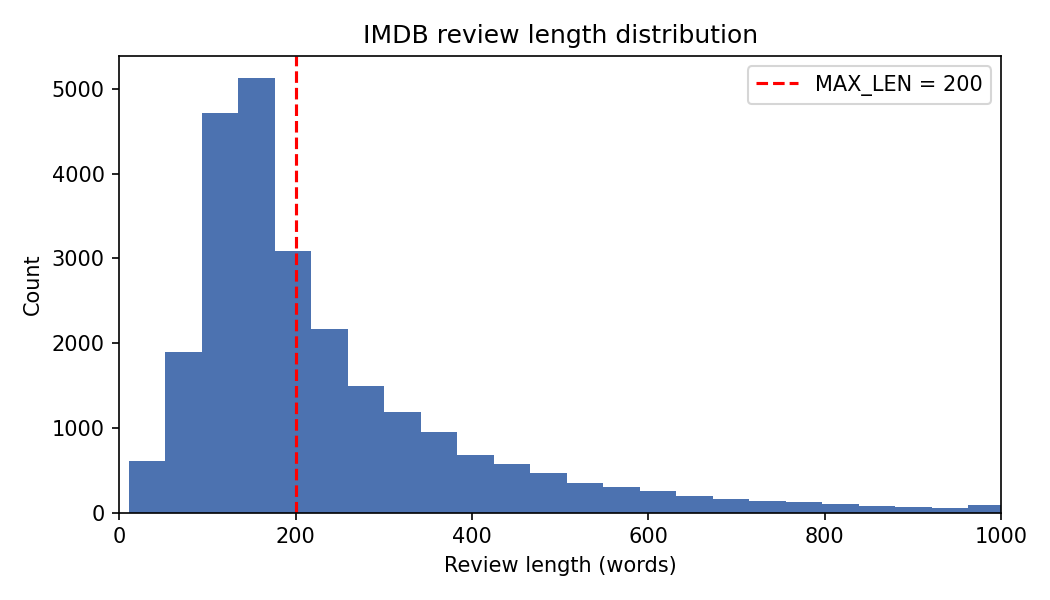
\includegraphics[width=\columnwidth]{fig0_review_lengths.png}}
\caption{Distribution of review lengths in the training set. The dashed line marks the chosen sequence length of 200.}
\label{fig:len}
\end{figure}

\subsection{Preprocessing}
Only the 10,000 most frequent words were kept, and the remaining words were mapped to an unknown token. Each word was converted to an integer index, and every review was padded or truncated to a fixed length of $T = 200$ tokens.

\subsection{Model Architectures}
All models share the pipeline: Input (200 tokens) $\rightarrow$ Embedding ($10{,}000 \times 64$) $\rightarrow$ recurrent layer (64 units) $\rightarrow$ Dropout (0.5)~\cite{srivastava2014} $\rightarrow$ Dense (1, sigmoid). Only the recurrent layer is changed.

\textbf{SimpleRNN:} The hidden state is updated as
\begin{equation}
h_t = \tanh(W_x x_t + W_h h_{t-1} + b).
\end{equation}

\textbf{LSTM:} A cell state $c_t$ is controlled by forget, input and output gates:
\begin{align}
f_t &= \sigma(W_f [h_{t-1}, x_t] + b_f) \\
i_t &= \sigma(W_i [h_{t-1}, x_t] + b_i) \\
o_t &= \sigma(W_o [h_{t-1}, x_t] + b_o) \\
\tilde{c}_t &= \tanh(W_c [h_{t-1}, x_t] + b_c) \\
c_t &= f_t \odot c_{t-1} + i_t \odot \tilde{c}_t \\
h_t &= o_t \odot \tanh(c_t)
\end{align}

\textbf{GRU:} Merges the cell and hidden state using update ($z_t$) and reset ($r_t$) gates:
\begin{align}
z_t &= \sigma(W_z [h_{t-1}, x_t]) \\
r_t &= \sigma(W_r [h_{t-1}, x_t]) \\
\tilde{h}_t &= \tanh(W [r_t \odot h_{t-1}, x_t]) \\
h_t &= (1 - z_t) \odot h_{t-1} + z_t \odot \tilde{h}_t
\end{align}

\textbf{BiLSTM:} Two LSTMs process the sequence forward and backward, and their final hidden states are concatenated, $h = [\overrightarrow{h}_T ; \overleftarrow{h}_1]$.

The output layer computes $\hat{y} = \sigma(w^\top h + b)$, which is the probability that the review is positive.

\subsection{Training Setup}
All models were trained with the Adam optimizer~\cite{kingma2015} and binary cross-entropy loss,
\begin{equation}
\mathcal{L} = -\frac{1}{N}\sum_{i=1}^{N} \left[ y_i \log \hat{y}_i + (1-y_i)\log(1-\hat{y}_i) \right],
\end{equation}
with batch size 128 and at most 5 epochs. Early stopping monitored the validation loss with patience 2 and restored the best weights. The random seed was fixed to 42. The implementation used Python 3.11, TensorFlow/Keras and scikit-learn, and training ran on a CPU. The models were evaluated using accuracy, precision, recall, F1-score, confusion matrices, training time and parameter count.

\section{Results and Discussion}

\begin{table}[htbp]
\caption{Performance on the IMDB Test Set (25,000 Reviews)}
\label{tab:results}
\centering
\setlength{\tabcolsep}{3.5pt}
\begin{tabular}{lcccccc}
\toprule
\textbf{Model} & \textbf{Params} & \textbf{Acc.} & \textbf{Prec.} & \textbf{Rec.} & \textbf{F1} & \textbf{Time (s)} \\
\midrule
SimpleRNN & 648,321 & 0.8312 & 0.8291 & 0.8344 & 0.8317 & \textbf{94.8} \\
LSTM      & 673,089 & \textbf{0.8676} & \textbf{0.8791} & 0.8526 & 0.8656 & 295.7 \\
GRU       & 665,025 & 0.8554 & 0.8567 & 0.8535 & 0.8551 & 272.0 \\
BiLSTM    & 706,177 & 0.8662 & 0.8596 & \textbf{0.8755} & \textbf{0.8675} & 536.9 \\
\bottomrule
\end{tabular}
\end{table}

Table~\ref{tab:results} summarises the test results, and Fig.~\ref{fig:metrics} compares the metrics visually.

\begin{figure}[htbp]
\centerline{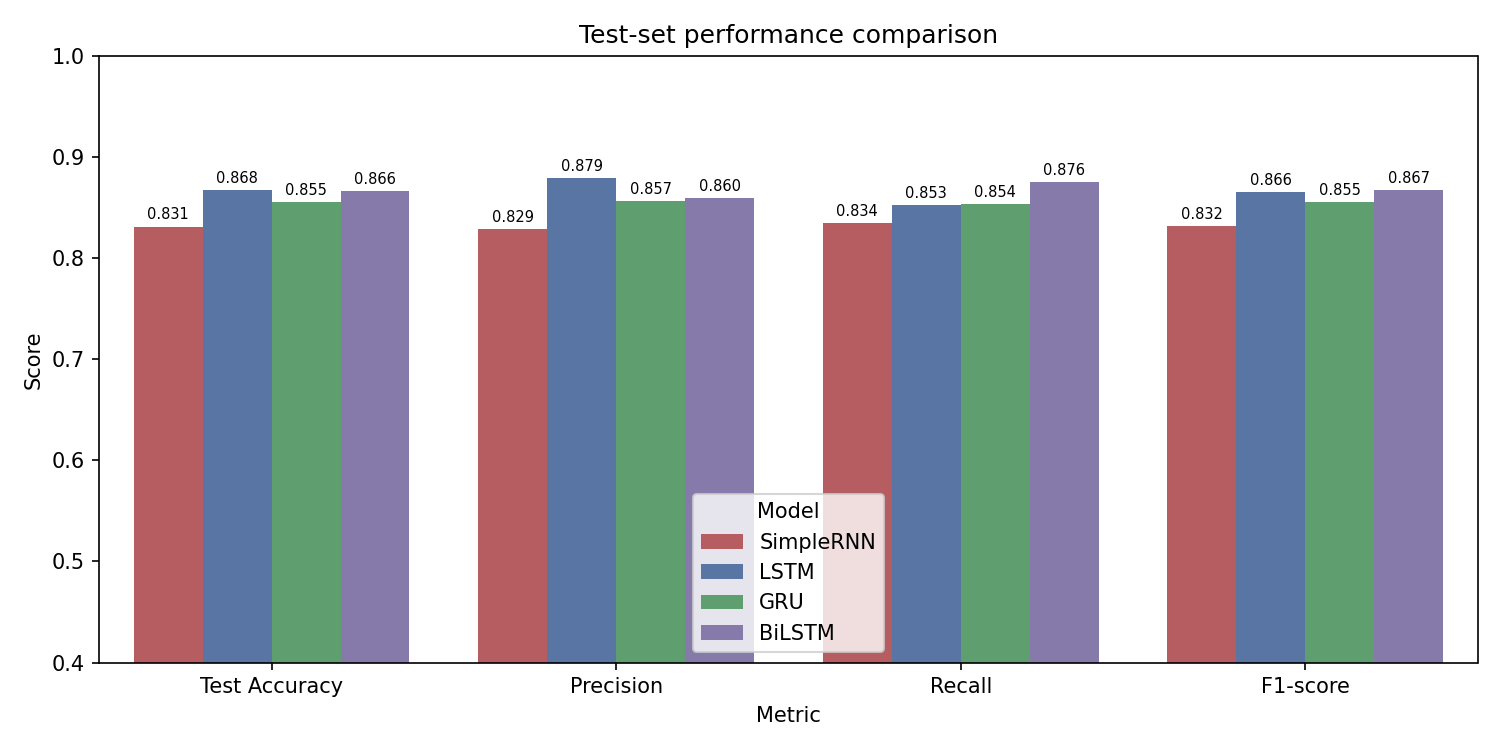
\includegraphics[width=\columnwidth]{fig2_metric_comparison.png}}
\caption{Test-set accuracy, precision, recall and F1-score of each model.}
\label{fig:metrics}
\end{figure}

\begin{figure*}[htbp]
\centerline{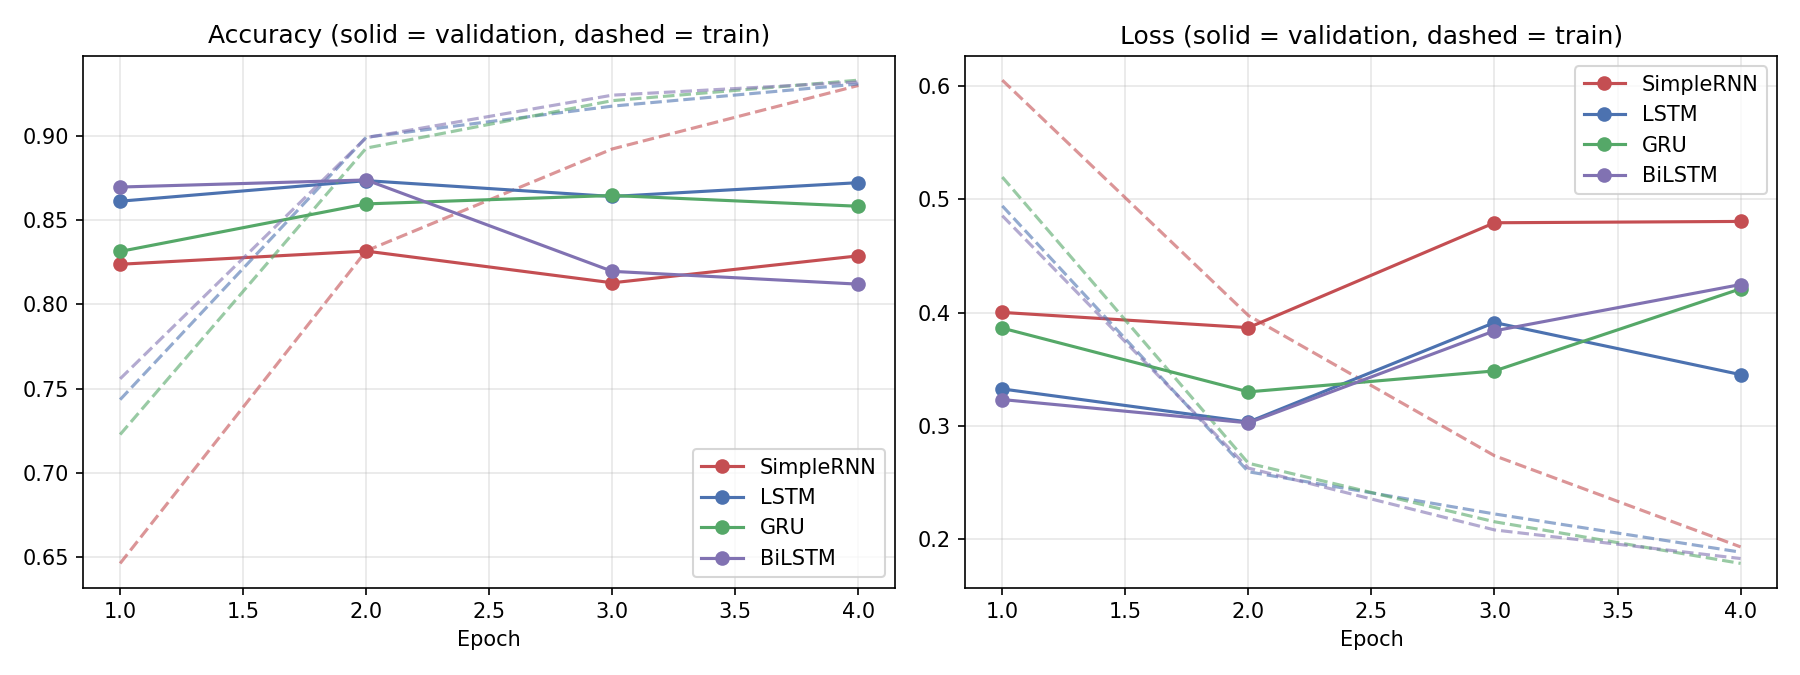
\includegraphics[width=0.85\textwidth]{fig1_training_curves.png}}
\caption{Training (dashed) and validation (solid) accuracy and loss per epoch.}
\label{fig:curves}
\end{figure*}

\begin{figure*}[htbp]
\centerline{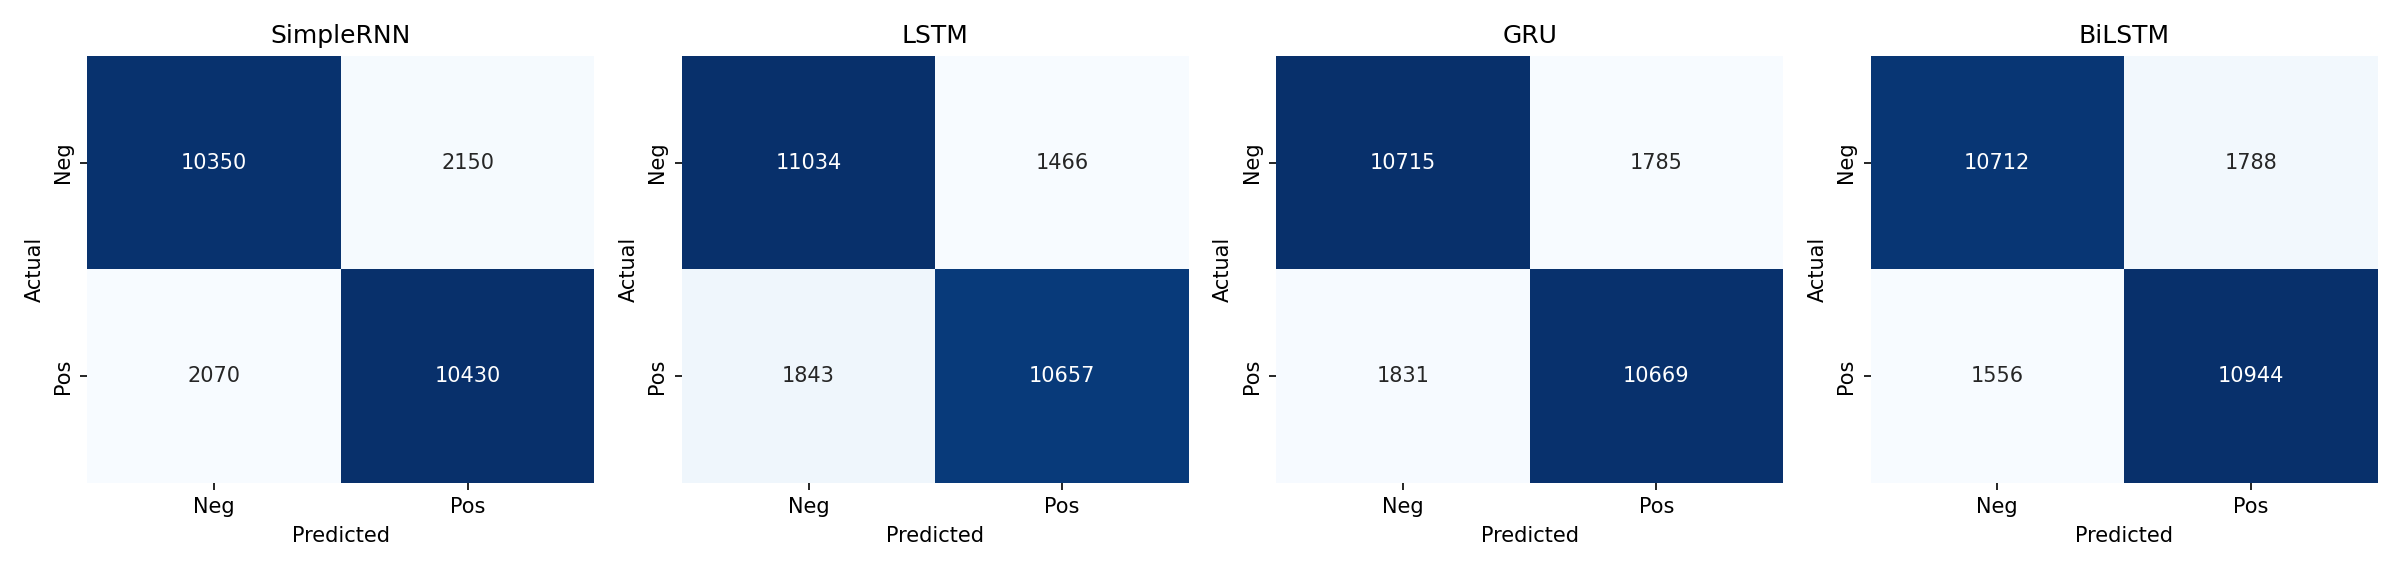
\includegraphics[width=0.95\textwidth]{fig3_confusion_matrices.png}}
\caption{Confusion matrices of the four models on the test set.}
\label{fig:cm}
\end{figure*}

\subsection{Effect of Gating}
All gated models outperform SimpleRNN by 2.4--3.6 percentage points in accuracy. This confirms that the forget and update gates preserve sentiment cues appearing early in long reviews, which the SimpleRNN loses due to vanishing gradients~\cite{bengio1994}.

\subsection{LSTM versus GRU}
LSTM is slightly more accurate than GRU (86.76\% vs.\ 85.54\%), while GRU uses fewer parameters and trains about 8\% faster. The small gap agrees with the findings of Chung \textit{et al.}~\cite{chung2014}, which makes GRU a good choice when resources are limited.

\subsection{Bidirectional Processing}
BiLSTM obtains the highest recall (0.876) and F1-score (0.867) but not higher accuracy than LSTM, and it needs $1.8\times$ the training time (Fig.~\ref{fig:time}). For whole-document classification, the additional backward context gives little benefit for its cost.

\begin{figure}[htbp]
\centerline{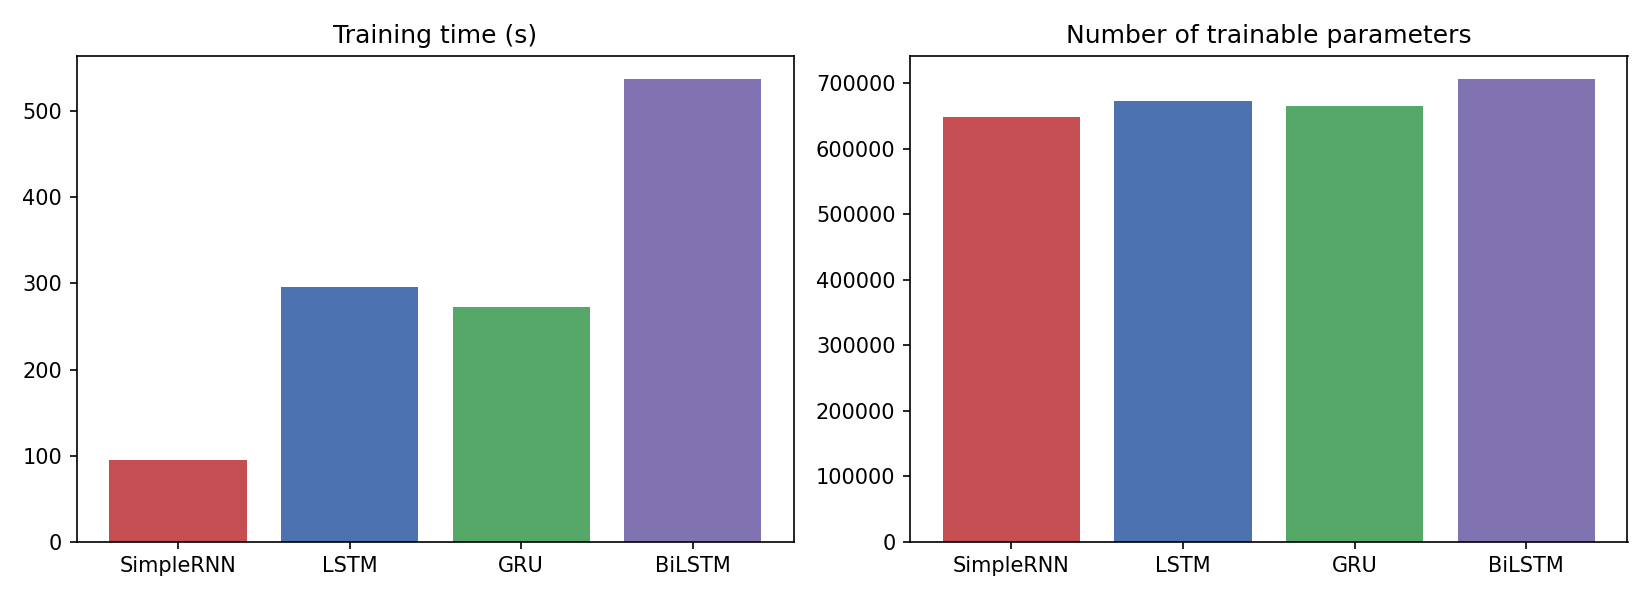
\includegraphics[width=\columnwidth]{fig4_time_and_params.png}}
\caption{Training time and number of trainable parameters.}
\label{fig:time}
\end{figure}

\subsection{Overfitting}
Fig.~\ref{fig:curves} shows that training accuracy keeps rising to about 93\%, while validation loss starts to increase after epoch 2 for every model. Early stopping restored the best weights, which shows that regularisation is necessary even for small recurrent models.

\subsection{Qualitative Analysis}
Table~\ref{tab:demo} shows the predictions for unseen sentences written by the authors. All models classify strongly polar reviews correctly. On the mixed review, only the gated models recognise that the clause after ``but'' dominates the sentiment. The negated sentence remains difficult: LSTM is borderline (0.51), which reveals a limitation in handling negation.

\begin{table}[htbp]
\caption{Predicted Probability of Positive Sentiment for New Reviews}
\label{tab:demo}
\centering
\setlength{\tabcolsep}{3pt}
\begin{tabular}{p{3.2cm}cccc}
\toprule
\textbf{Review} & \textbf{RNN} & \textbf{LSTM} & \textbf{GRU} & \textbf{BiLSTM} \\
\midrule
``Absolutely wonderful, acting was brilliant'' (+) & 0.62 & 0.94 & 0.94 & 0.92 \\
``Worst film \ldots\ complete waste of time'' ($-$) & 0.01 & 0.01 & 0.00 & 0.01 \\
``Plot was predictable but music and visuals were great'' (+) & \textcolor{red}{0.27} & 0.71 & 0.67 & 0.61 \\
``I did not like this movie, it was not good'' ($-$) & 0.08 & \textcolor{red}{0.51} & 0.45 & 0.36 \\
\bottomrule
\end{tabular}
\end{table}

\section{Conclusion and Future Work}
This paper compared four recurrent architectures for sentiment analysis on the IMDB dataset under identical settings. Gated models clearly outperform the basic RNN, and LSTM achieved the best accuracy of 86.76\%. GRU offers nearly the same accuracy with fewer parameters and less training time, which makes it suitable for resource-constrained deployment, while BiLSTM did not justify its doubled training cost for this task. Future work includes pretrained embeddings (GloVe, Word2Vec), attention mechanisms, comparison with Transformer models such as BERT~\cite{devlin2019}, aspect-based sentiment analysis, and multiple random seeds to test the statistical significance of the observed differences.

\begin{thebibliography}{00}
\bibitem{maas2011} A. L. Maas, R. E. Daly, P. T. Pham, D. Huang, A. Y. Ng, and C. Potts, ``Learning word vectors for sentiment analysis,'' in \textit{Proc. 49th Annu. Meeting Assoc. Comput. Linguistics (ACL)}, 2011, pp. 142--150.
\bibitem{hochreiter1997} S. Hochreiter and J. Schmidhuber, ``Long short-term memory,'' \textit{Neural Computation}, vol. 9, no. 8, pp. 1735--1780, 1997.
\bibitem{cho2014} K. Cho \textit{et al.}, ``Learning phrase representations using RNN encoder--decoder for statistical machine translation,'' in \textit{Proc. EMNLP}, 2014, pp. 1724--1734.
\bibitem{chung2014} J. Chung, C. Gulcehre, K. Cho, and Y. Bengio, ``Empirical evaluation of gated recurrent neural networks on sequence modeling,'' arXiv:1412.3555, 2014.
\bibitem{schuster1997} M. Schuster and K. K. Paliwal, ``Bidirectional recurrent neural networks,'' \textit{IEEE Trans. Signal Process.}, vol. 45, no. 11, pp. 2673--2681, 1997.
\bibitem{bengio1994} Y. Bengio, P. Simard, and P. Frasconi, ``Learning long-term dependencies with gradient descent is difficult,'' \textit{IEEE Trans. Neural Netw.}, vol. 5, no. 2, pp. 157--166, 1994.
\bibitem{devlin2019} J. Devlin, M.-W. Chang, K. Lee, and K. Toutanova, ``BERT: Pre-training of deep bidirectional transformers for language understanding,'' in \textit{Proc. NAACL-HLT}, 2019, pp. 4171--4186.
\bibitem{kingma2015} D. P. Kingma and J. Ba, ``Adam: A method for stochastic optimization,'' in \textit{Proc. ICLR}, 2015.
\bibitem{srivastava2014} N. Srivastava, G. Hinton, A. Krizhevsky, I. Sutskever, and R. Salakhutdinov, ``Dropout: A simple way to prevent neural networks from overfitting,'' \textit{J. Mach. Learn. Res.}, vol. 15, pp. 1929--1958, 2014.
\end{thebibliography}

\end{document}
